\documentclass{beamer}

\usetheme{Copenhagen}

\title{Cornu Spirals}
\subtitle{From Euler to Ferrari}
\author{Max Mussavian}
\logo{
\includegraphics[height=1.5cm]{Tonbridge_School_logo.png}}
\date[2022]{Arcana, May 2022}
\begin{document}
\begin{frame}[plain]
    \maketitle
\end{frame}
\begin{frame}{Outline}
	\begin{itemize}
		\item Definitions: Curves, Lengths and Curvature
		\item Relating the Curve Length to its Curvature
		\item The Euler Spiral
		\item Other Fun Curves
		\item ``Curvature determines the Curve''
		\item Application 1: Designing Roads and Railways
		\item Application 2: The Racing Line
	\end{itemize}
\end{frame}

\begin{frame}{What is a Curve?}
	Before we begin note that everything we look at here is in 2 dimensions $\mathbb{R}^2$
	\begin{definition}[A Parametric Curve]
		A parametric curve is a twice differentiable function that has the form
		$x = g(t)$ and $y=h(t)$ defined on an open interval $(a, b)$.
		
		The set of points traced out by the curve is called the trace.
	\end{definition}
\end{frame}

\begin{frame}{How Long is a Curve?}
	\begin{definition}[Arc Length]
		The length of a curve $s$ is given by
		$s = \int_{t_1}^{t_2} \sqrt{x'^2+y'^2}dt$
	\end{definition}
	Intuition: The velocity at time $t$ is $\left( \begin{array}{c}
		x'(t)\\
		y'(t)
	\end{array} \right)$ and hence the speed at time $t$ is $\sqrt{x'(t)^2+y'(t)^2}$. Distance travelled (arc length) is the integral of speed with respect to time. 

	Alternatively approximate the trace by line segments. The length of line segments converges to the arc length as the segments get smaller and smaller.
\end{frame}

\begin{frame}{Some Simple Examples}
\begin{itemize}
	
	\item Circle: We can define a circle with radius $r$ as $x(t)=r \cos(t)$ and $y(t)= r \sin(t)$. The arc length is 
	\[
	s = \int_{0}^{2 \pi} \sqrt{r^2 \sin^2 t + r^2 \cos^2 t}dt = \left[r \right]_{0}^{2 \pi} = 2 \pi r
	\]
	
	\item Parabola: We can define a parabola as $x(t)=t$ and $y(t)=t^2$. The Arc Length between 0 and 1 is 
	\begin{eqnarray*}
	s &=& \int_{0}^{1} \sqrt{1+4t^2}dt \\ &=& \left[\frac{1}{2} t\sqrt{1+ 4 t^2} +\frac{1}{4} \ln \left(2 t+\sqrt{1+ 4 t^2} \right) \right]_{0}^1 \\
	&\approx&	 1.48
	\end{eqnarray*}
\end{itemize}

\end{frame}

\begin{frame}{How Curved is a Curve?}
	The curvature at a point on the curve is the reciprocal of the radius of the circle that approximates the curve.
	\begin{definition}[Curvature]
		The curvature of curve is $\kappa$ given by
		$\kappa=\frac{x' y'' - y' x''}{(x'^2+y'^2)^{3/2}}$
	\end{definition}
	Note: Curvature is signed in two dimensions. Positive curvature corresponds ``bending to the left'' while negative curvature ``bends to the right''.
\end{frame}

\begin{frame}{Explaining Definition for Curvature}
	\begin{columns}
		\begin{column}{0.4\textwidth}
			\begin{figure}
				\centering
				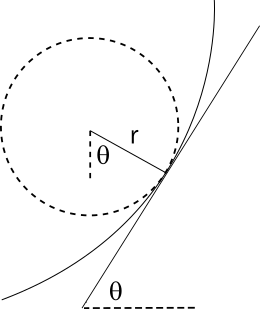
\includegraphics[width=50mm, scale=0.5]{illustration.png}
			\end{figure}
		\end{column}
		\begin{column}{0.6\textwidth}
			For any circle with radius $r$ we have $s=r \theta$.
			
			Therefore for ``kissing'' circle 
			$\frac{ds}{dt} = r \frac{d\theta}{dt}$
			
			But $\tan \theta = \frac{y'(t)}{x'(t)}$ and taking derivatives w.r.t. $t$ we have $\sec ^2 \theta \frac{d\theta}{dt} = \frac{x' y'' - y' x''}{x'^2}$.
			
			Further $\frac{1}{\cos^2 \theta} = \frac{x'^2+y'^2}{x'^2}$ therefore
			$\frac{d\theta}{dt}=\frac{x' y'' - y' x''}{x'^2+y'^2}$
			
			From above $\frac{ds}{dt} = \sqrt{x'^2+y'^2}$.
			
			Combing gives us
			$r= \frac{ds/dt}{d\theta/dt} =\frac{(x'^2+y'^2)^{3/2}}{x' y'' - y' x''}$
			
			Finally note $\kappa = \frac{1}{r}$
			
			
			
		\end{column}
	\end{columns}

	
\end{frame}

\begin{frame}{Some Simple Examples}
	\begin{itemize}	
		\item Circle: Recall $x(t)=r \cos(t)$ and $y(t)= r \sin(t)$ 
		\[
		\kappa = \frac{r^2 \sin^2 t + r^2 \cos^2 t}{\left(r^2 \sin^2 t + r^2 \cos^2 t \right) ^ \frac{3}{2}} = \frac{1}{r}
		\]
		
		\item Parabola: Recall $x(t)=t$ and $y(t)=t^2$. 
		
		\[
		\kappa = \frac{2}{\left(1 + 4t^2 \right) ^ \frac{3}{2}}
		\]
	\end{itemize}
\end{frame}

\begin{frame}{Relating Curve Length to Curvature}
	Let's try the following parametrisation for $x$ and $y$
	\begin{eqnarray*}
		x(t) &=& \int_{0}^{t} \cos f(u) du \\
		y(t) &=& \int_{0}^{t} \sin f(u) du
	\end{eqnarray*}
	This gives us
	\begin{eqnarray*}
		x' = x'(t) = \cos f(t) &\mbox{ and }& x''=-f'(t) \sin f(t) \\
		y' = y'(t) = \sin f(t) &\mbox{ and }& y''=f'(t) \cos f(t)
	\end{eqnarray*}
\end{frame}

\begin{frame}{Relating Curve Length to Curvature}
	This gives us the following for slope, arc length and curvature
	\begin{eqnarray*}
	\frac{dy}{dx} &=& \frac{\sin f(t)}{\cos f(t)} = \tan f(t) \\
 	s &=& \int_0^t \sqrt{\cos^2 f(u) + \sin^2 f(u)} du = t \\
 	\kappa &=& \frac{f'(t) \cos^2 f(t) + f'(t) \sin^2 f(t)}{\cos^2 f(t) + \sin^2 f(t)} = f'(t)
 \end{eqnarray*}
\end{frame}

\begin{frame}{Define the Curve by Curve Length and Curvature}
	We can get replace ``time'' variable $t$ by the curve length $s$.
	 
	And the curvature at point $t$ is $f'(t)$. Which means
	 \[
	 f(t) = \int \kappa(t) dt
	 \]
	Thus the equations for the curve become
	\begin{eqnarray*}
	x = x(s) &=& \int_{0}^{s} \cos \left( \int_0^u \kappa(t) dt \right) du \\
	y = y(s) &=& \int_{0}^{s} \sin \left( \int_0^u \kappa(t) dt \right) du
	\end{eqnarray*}
	Hence the curve is defined by curve length and curvature alone.
\end{frame}

\begin{frame}{A Very Simple Example}
	We can make the curvature $\kappa$ constant and equal to 1. Then 
	$ \int_0^u \kappa(t) dt = u $ and
	\begin{eqnarray*}
		x = x(s) &=& \int_{0}^{s} \cos u du = \sin s\\
		y = y(s) &=& \int_{0}^{s} \sin u du = - \cos s + 1
	\end{eqnarray*}
	which is the parametric curve for a circle with centre $(0, 1)$ and radius $1$.
	
\end{frame}


\begin{frame}{The Euler Spiral}
	A more interesting example is the curvature equal to the arc length. 
	
	\begin{center}
		\boxed{\kappa(s) = s}
	\end{center}
	Then 
	$ \int_0^u \kappa(t) dt = \frac{u^2}{2} $ and
	\begin{eqnarray*}
		x = x(s) &=& \int_{0}^{s} \cos \frac{u^2}{2} du\\
		y = y(s) &=& \int_{0}^{s} \sin \frac{u^2}{2} du
	\end{eqnarray*}
	These integrals are called ``Fresnel Integrals''. 
	
	They cannot be solved analytically. But what do they look like numerically?
\end{frame}

\begin{frame}{Making a Plotter in Python}
	\begin{columns}
		\begin{column}{0.5\textwidth}
			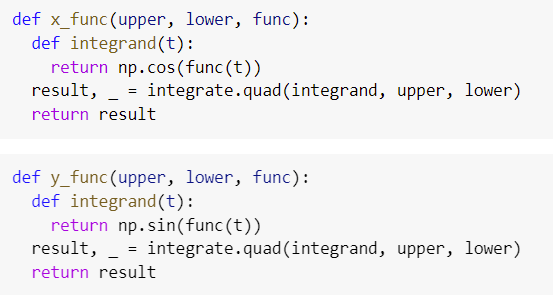
\includegraphics[width=50mm, scale=0.5]{code_1.png}
			
			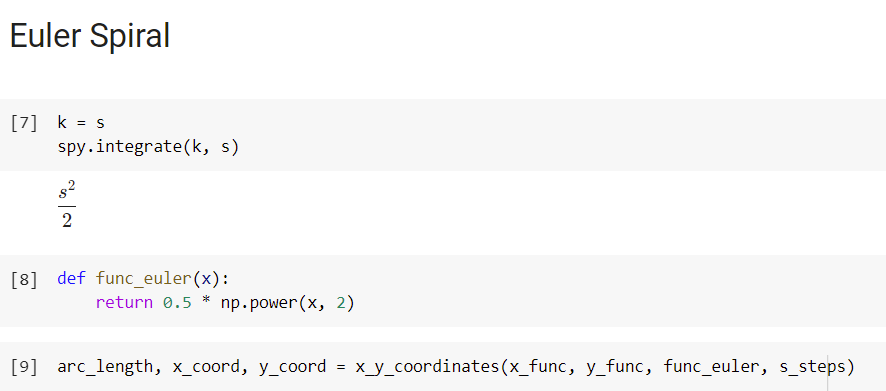
\includegraphics[width=50mm, scale=0.5]{code_2.png}
		\end{column}
		\begin{column}{0.5\textwidth}
			First write functions to calculate x and y coordinates 
			More words here
			
		\end{column}
	\end{columns}
\end{frame}


\begin{frame}{The Euler Spiral}
	\begin{figure}
		\caption{The Euler Spiral aka Cornu Curve}
		\centering
		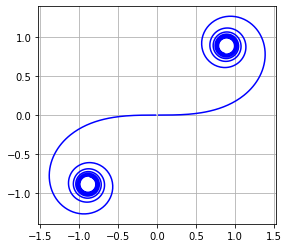
\includegraphics[width=70mm, scale=0.5]{euler_spiral.png}
	\end{figure}
	
\end{frame}

\begin{frame}{The Euler Spiral - $x$ $y$ Coordinates}
	\begin{figure}
	\caption{Fresnel Integrals with arguments $\frac{u^2}{2}$}
	\centering
	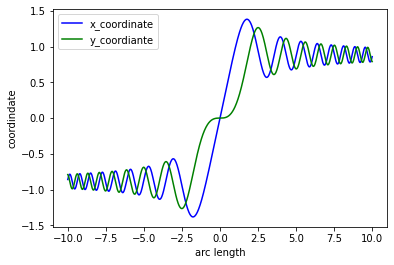
\includegraphics[width=70mm, scale=0.5]{euler_x_vs_y.png}
	\end{figure}
	These converge to $\pm \frac{\sqrt{\pi}}{2} \approx 0.8862$.
\end{frame}

\begin{frame}{Other Fun Curves: Even Powers of $s$}
	\begin{figure}
		\caption{$\kappa(s) = s^2$}
		\centering
		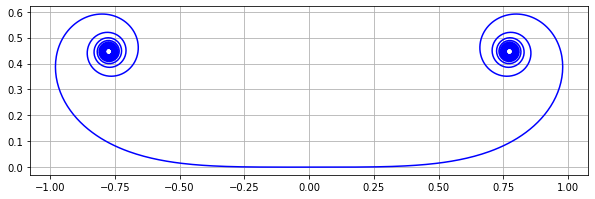
\includegraphics[width=85mm, scale=0.5]{chaise_longue.png}
	\end{figure}
\end{frame}

\begin{frame}{More Fun Curves: Mix in a Bit of a Circle}
	\begin{figure}
		\caption{$\kappa(s) = s ^ 2 -2.19$}
		\centering
		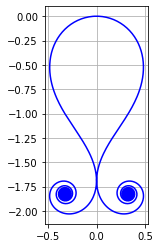
\includegraphics[width=35mm, scale=0.2]{s_squared_minus_219.png}
	\end{figure}
\end{frame}

\begin{frame}{More Fun Curves: Polynomials}
	\begin{figure}
		\caption{$\kappa(s) = 5 s ^ 4 - 18 s ^ 2 + 5$}
		\centering
		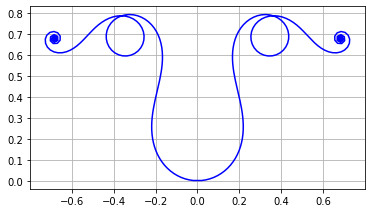
\includegraphics[width=70mm, scale=0.5]{five_s^4.png}
	\end{figure}
\end{frame}

\begin{frame}{More Fun Curves: Trigonometric Functions}
	\begin{figure}
		\caption{$\kappa(s) = \cos(s) - s \sin(s)$}
		\centering
		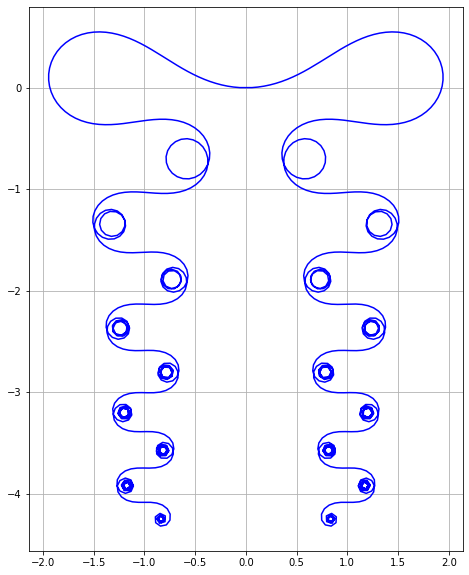
\includegraphics[width=50mm, scale=0.2]{elegant_madness.png}
	\end{figure}
\end{frame}
	
\begin{frame}{More Fun Curves: Hyperbolic Functions}
	\begin{figure}
		\caption{$\kappa(s) = \sinh(s) - 5.19$}
		\centering
		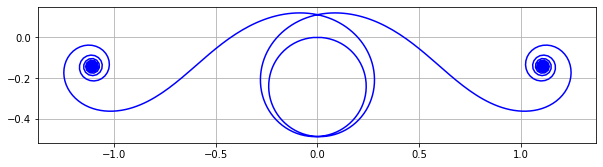
\includegraphics[width=100mm, scale=0.5]{sinh.png}
	\end{figure}
\end{frame}


\begin{frame}{"Curvature determines the Curve"}
	
\end{frame}

\begin{frame}{Diffraction and Fresnel Integrals}
	
\end{frame}

\begin{frame}{Designing Roads and Railways}
	\begin{enumerate}
		\item Transition curves are used to link straight sections of motorways or railways.
		\item They are designed to give passengers a smooth ride.
		\item In particular so sudden changes in acceleration.

	\end{enumerate}
		\begin{figure}
		\caption{Cloverleaf Motorway Interchange}
		\centering
		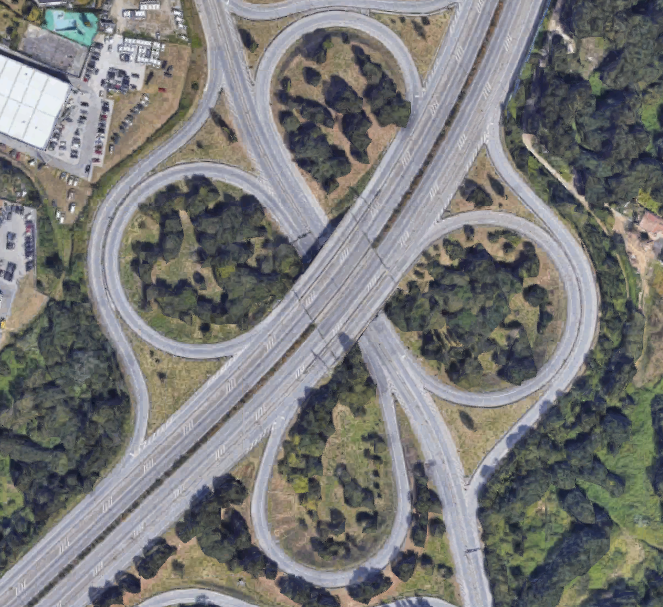
\includegraphics[width=20mm, scale=0.5]{cloverleaf_motorway.png}
	\end{figure}

\end{frame}

\begin{frame}{Why Transition Curves are Euler Spirals}
	\begin{itemize}
	\item The acceleration along the transition is given by
 	 \[
 	 a=s''(t) \vec{T}+\kappa s'(t)^2 \vec{N}
 	 \]
 	 Where $\vec{T}$ is the unit tangent vector and $\vec{N}$ is the unit normal vector.
 	 \item If the car/train is going round the curve at constant speed $s'(t)=constant$ and $s''(t)=0$.	
 	 \item The acceleration at constant speed only depends on the curvature $\kappa$ and speed $s'(t)$ in the direction of the normal vector.
\end{itemize}

\end{frame}

\begin{frame}{The Racing Line}
	
\end{frame}




\end{document}
